\chapter{Background}

\textit{Cos'è la vita? Da dove viene?} - Fino al 18° secolo per rispondere a tale quesito si faceva riferimento alla fede nel vitalismo: l'esistenza di una forza vitale non subordinata a leggi della chimica e  della fisica.
Il cambiamento avvenne nel 19° secolo.
Un'importante svolta fu il lavoro di Louis Pasteur che stabilì un collegamento fra processi vitali e reazioni chimiche: la conversione di zucchero in alcool (fermentazione) era un risultato della crescita di microorganismi.
\par Successivamente vi sono i lavori di Berthelot e Buchner (premio Nobel per la Chimica 1907), il quale dimostrò che era possibile ottenere la fermentazione in assenza di microorganismi, usando solamente sostanze estratte da essi.
Queste sostanze furono chiamate \textit{enzimi} (dal ted. Enzym, letteralmente «dentro il lievito»\supercite{enzimaTreccani}). Non si conosceva la loro natura chimica, si scoprì successivamente che tutti gli enzimi sono \textit{proteine} (dal greco «primario», «che occupa la prima posizione» \supercite{proteinaTreccani}).
Queste proteine agivano da catalizzatori: acceleravano le reazioni chimiche all'interno delle cellule e nei tessuti senza cambiare la loro natura, quindi senza consumarsi, e senza entrare nei prodotti finali della reazione.

\par La scoperta degli enzimi portò ad un cambio di paradigma nel pensiero scientifico riguardo le origini della vita: veniva ora considerata come la conseguenza di numerosi processi chimici resi possibili dalle proteine \supercite{kessel_ben-tal_2018}.
I fondamenti del pensiero biologico si spostarono dal vitalismo al meccanicismo secondo il quale tutti i fenomeni naturali, vita compresa, sono governati dalle stesse leggi, sia per sostanze organiche che inorganiche.

\par L'inconorazione delle proteine a \textit{macromolecole più importanti della vita} si può legare ad un'altra svolta nel pensiero scientifico avvenuta nella seconda metà del 20° secolo: la rivoluzione genetica. 
Le proteine sono ben più che "macchine molecolari": sono i prodotti primari dei geni, responsabili, fra altri, dell'espressione dell'informazione genetica. È sullo sfondo di questa rivoluzione che l'informatica si è inserita all'interno del mondo della biologia.

\clearpage

\section{Background biologico}
\subsection{Organizzazione della vita: dagli atomi alle cellule}
Nonostante le grandi differenze in dimensione, dieta, riproduzione, morfologia, comportamento, vi è un tratto comune a tutti gli organismi viventi: sono composti di cellule. Tutte le cellule sono caratterizzate da una stupefacente somiglianza chimica poiché utilizzano molecole simili e hanno ereditato tutte le stesse intuizioni genetiche. Si pensa quindi vi sia un antenato comune a tutti i viventi: una cellula vissuta circa 3,5 miliardi di anni fa che conteneva un prototipo del macchinario universale della vita sulla Terra oggi \supercite{alberts2018essential}. \\

\par Prima di parlare di cellule è opportuno richiamare l'attenzione sulle strutture biologiche. L'organizzazione biologica si basa su una gerarchia di livelli strutturali \footnote{Questa sezione di background biologico si basa in larga parte sui personali \fullcite{EBN}, frequentato nell'a.a. 2020/21 come esame a libera scelta.}, ognuno dei quali poggia su un gradino sottostante: 

\begin{figure}[h]
	\centering
	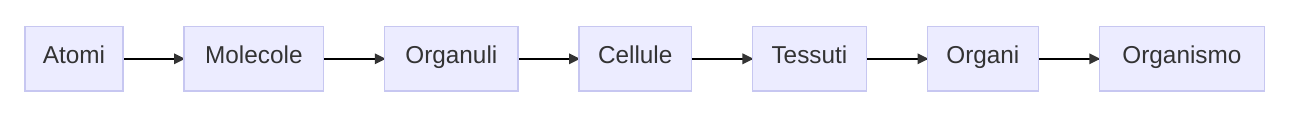
\includegraphics[scale=0.45] {images/strutture_biologiche.png}
\end{figure}


\par Tutta la materia è costituita da 94 elementi chimici in natura (tralasciando quelli non stabili). La materia organica è composta per il 96\% da atomi di C, O, N, H (carbonio, ossigeno, azoto, idrogeno). Un atomo ha un nucleo composto da neutroni e protoni circondato da una nube di elettroni in rapido movimento. Il Dalton (Da) è l'unità della massa atomica, corrisponde al peso di un protone o neutrone: $1 Da = 1.7 \times 10^{-24}g$. Un elettrone pesa $0.0005 Da$. Gli elettroni più esterni sono chiamati \textit{elettroni di valenza} e determinano il comportamento chimico di un atomo.

\par Lo scheletro dei composti organici è formato da catene carboniose, lunghe catene di atomi di carbonio legati fra loro da legami covalenti (il tipo di legame chimico più forte). Salendo di un livello nella gerarchia strutturale si arriva alle macromolecole biologiche, fondamentali per le cellule: carboidrati, lipidi, acidi nucleici e proteine. I carboidrati sono combustibili cellulari e materiale da costruzione, i lipidi sono sia depositi di energia che gusci protettivi, gli acidi nucleici permettono di codificare l'informazione genica e le proteine sono alla base delle funzioni vitali.\\

La cellula è la più piccola unità in grado di vivere. Per \textit{vivente} si intende un essere dotato di: organizzazione interna, metabolismo, omeostasi, interazione con l'ambiente, adattamento, crescita e riproduzione.

\par Le cellule hanno dimensioni che variano dai 2$\mu m$ ai $cm$ delle uova di rana, gallina o struzzo ai $m$ di neuroni con lunghi assoni:

\begin{figure}[!h]
	\centering
	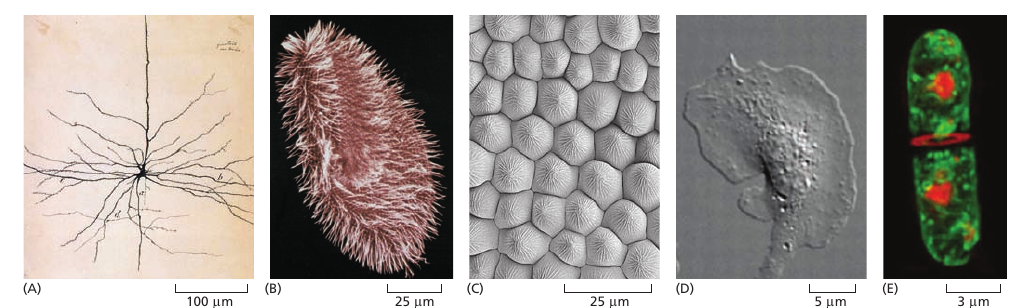
\includegraphics[scale=0.5] {images/cellule-dimensioni.png}
	\caption{(A) disegno di un neurone. (B) Paramecium. (C) superficie di un petalo di fiore di bocca di leone. (D) Macrofago. (E) Un lievito di fissione viene catturato nell'atto di divisione cellulare. Fonte: \cite{alberts2018essential}}
	\label{fig:cellule-dimensioni}
\end{figure}

\par È possibile dividere gli esseri viventi in due domini: \textit{procarioti} ed \textit{eucarioti}. Il primo include i due regni Bacteria e Archaea. Sono caratterizzati da cellule piccole, circa 1$\mu m$. Il secondo dominio include cinque regni: animali, piante, funghi, protisti e cromisti. Dispongono di cellule più grandi (circa 10-100 $\mu m$) dotate di compartimenti interni che dividono i processi cellulari.

La struttura tipica di una cellula animale è mostrata nella seguente figura:

\begin{figure}[!h]
	\centering
	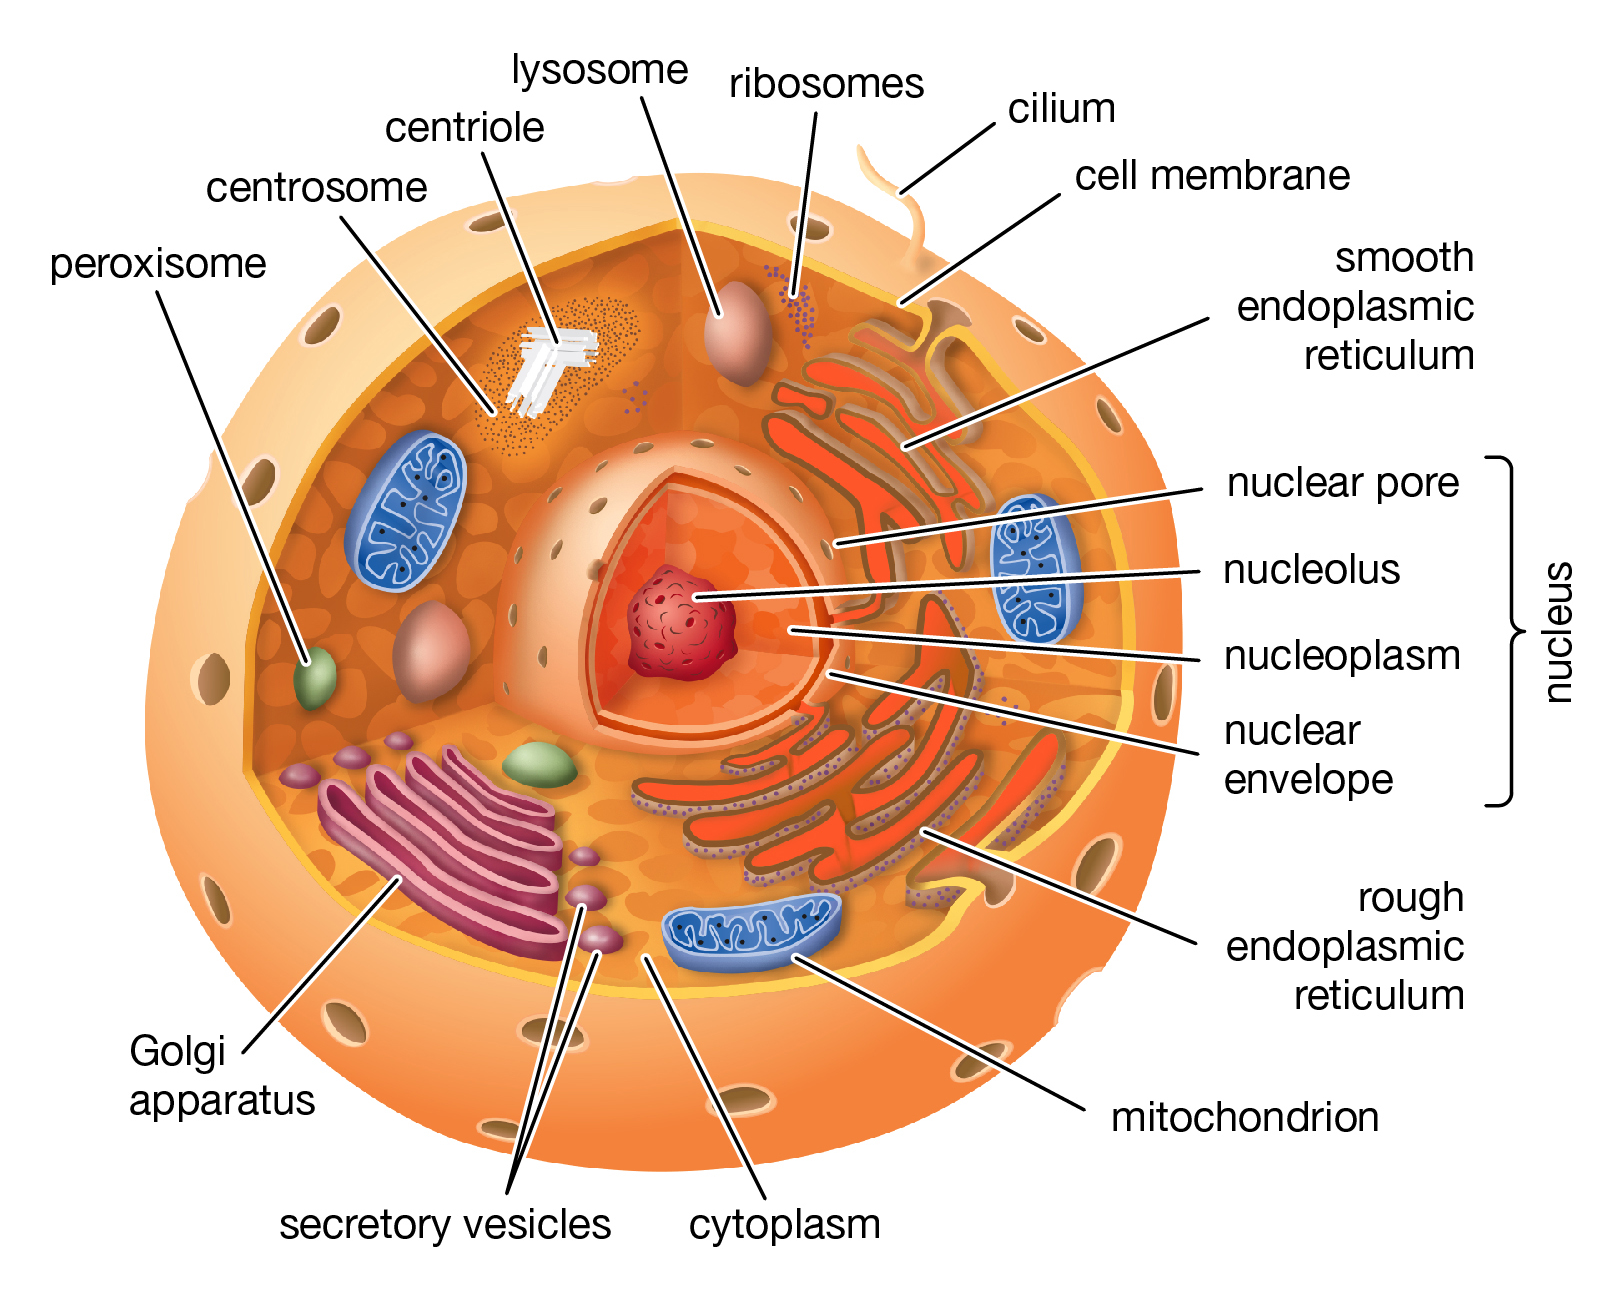
\includegraphics[scale=0.17]{images/cellula-eucariotica2.png}
	\caption{Cellula animale. Fonte: \cite{eukaryoteBritannica}}
	\label{fig:cellula-animale}
\end{figure}

L'interno delle cellule è composto da ambiente acquoso per il 70-95\%. \\

- completa con vita e funzionamento basilare, senza DNA \\

Il ciclo di vita delle cellule si basa su 4 fasi: crescita, sintesi del DNA, crescita completa e mitosi (divisione cellulare). Le cellule dei mammiferi impiegano da 18 a 24 ore per completare un ciclo di mitosi, mentre i lieviti solamente 90 minuti. Per questa ragione il lievito da fornaio (\textit{Saccharomyces cerevisiae}) è usato come organismo modello in citologia e genetica: il suo genoma è stato il primo ad essere sequenziato completamente tra gli eucarioti \supercite{lievitoWiki}. 

\par Le cellule hanno una durata di vita molto variabile, ad esempio alcuni organismi unicellulari come le spore possono vivere anche decenni, così come i nostri neuroni, mentre i globuli bianchi vengono ricambiati ogni 2 giorni. \\

\par Gli strumenti utilizzati per indagare nel mondo microscopico riescono a mostrare dettagli che vanno dal limite di 200$nm$ del microscopio ottico (limite imposto dalla natura ondulatoria della luce) alla precisione di 1$nm$ del microscopio a trasmissione elettronica (che usa fasci di elettroni invece di fasci di luce):

\begin{figure}[!h]
	\centering
	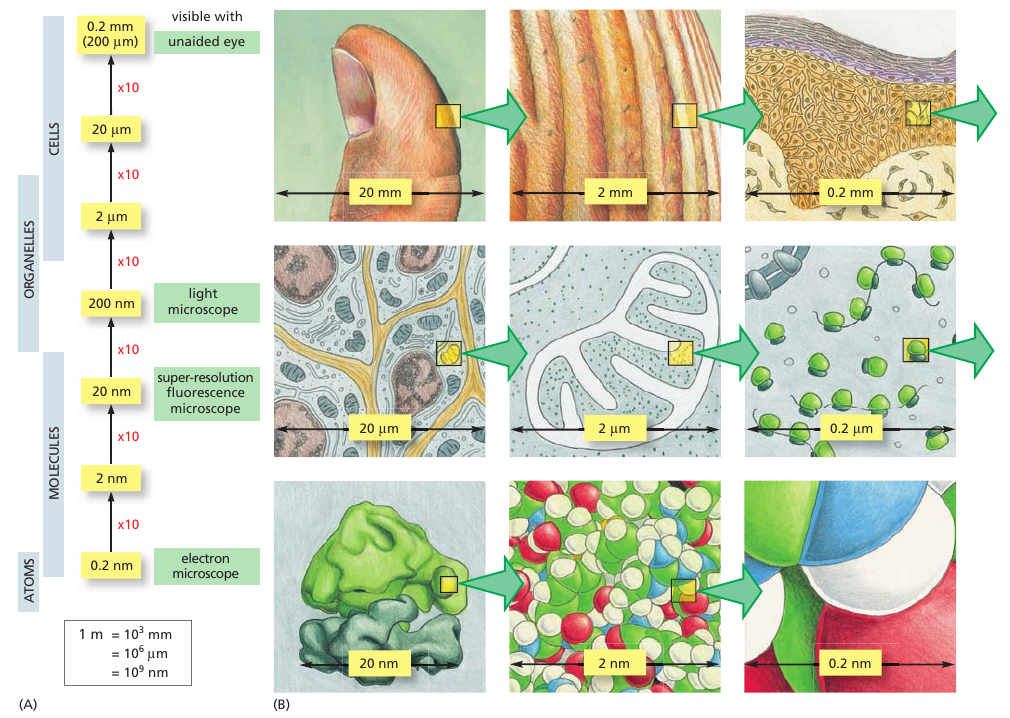
\includegraphics[scale=0.6]{images/grandezze.png}
	\caption{(A) Il grafico elenca le dimensioni dei livelli strutturali biologici, le unità di misura relative e gli strumenti necessari per visualizzarli. (B) Uno stesso dettaglio a varie scale di grandezza: pollice, pelle, cellule, mitocondrio, ribosomi, insieme di atomi che formano parte di una proteina. I dettagli molecolari sono oltre la potenza del microscopio elettronico. Fonte: \cite{alberts2018essential}}
	\label{fig:microscopi-grandezze}
\end{figure}

\subsection{Concetti fondamentali in biologia}

\begin{itemize}
	\item \textit{Proprietà emergenti }\\
			Ad ogni livello di indagine, ovvero passando da un livello della gerarchia strutturale al superiore, si palesano nuove proprietà non riconducibili ai livelli più semplici: le proprietà emergenti. Una singola molecola d'acqua non è né solida né liquida.
	\item \textit{Teoria cellulare} \\
			Le cellule rappresentano le unità strutturali e funzionali degli organismi.
	\item \textit{Geni} \\
			Il perpetuarsi della vita è possibile grazie alla trasmissione dei geni.
	\item \textit{Forma e funzione} \\
			Forma e funzione sono correlate a tutti i livelli biologici. Se le ali degli uccelli non fossero così come sono essi non potrebbero volare, se i mitocondri non avessero striature non potrebbero svolgere la respirazione cellulare, se i neuroni non avessero lunghi assoni non riuscirebbero a comunicare oppure si pensi al \textit{paramecium} che si muove come un sommergibile grazie alle sue ciglia (vedi figura \ref{fig:cellule-dimensioni}B).
	\item \textit{Evoluzione} \\
			L'evoluzione rappresenta il tema centrale ed unificante della biologia, come si è già accennato sopra. Gli organismi sono sistemi aperti che interagiscono continuamente con l'ambiente, dotati di variabilità individuale e finalizzati alla competizione per la sopravvivenza. 
	\item \textit{Diversità e unità} \\
			Vi sono da 5 a 30 milioni di specie differenti eppure scendendo sempre di più nella struttura degli organismi si osserva una similitudine quasi sconcertante. Un esempio che ci riguarda è la somiglianza fra le ciglia di \textit{paramecium} e le ciglia di una cellula epiteliale delle vie aeree degli esseri umani: presentano la stessa sezione trasversale. Diversità e unità della vita sulla Terra sono due facce della stessa medaglia.
			- somiglianza nel DNA e implicazioni per informatica - 
			
\end{itemize}

\subsection{Dogma centrale della biologia}
• DNA, fenotipo e genotipo
• RNA

Il DNA nel nucleo è associato a delle proteine con cui forma un materiale fibroso chiamato cromatina, mostrandosi "sfilacciato" in modo da poter essere letto. Quando la cellula si riproduce tali fibre si ispessiscono divenendo visibili come strutture compatte e singole: i cromosomi. Il nucleolo non è provvisto di membrana e serve per la sintesi di RNA ribosomiale, cioè l'RNA che uscendo dai pori dell'involucro nucleare andrà nel citoplasma a formare i ribosomi. Dall'involucro nucleare può uscire RNA e proteine ma non il DNA attraverso i pori presenti su di esso. L'RNA uscirà e andrà nel citoplasma per dirigere la sintesi proteica.

genoma: indica patrimonio complessivo del DNA di una cellula

\par

\begin{figure}[!htb]
	\minipage{0.5\textwidth}
	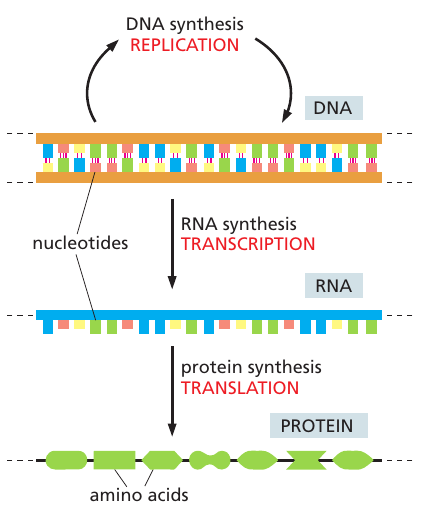
\includegraphics[scale=0.45]{images/central-dogma.png}
	\caption{Dogma centrale in biologia}\label{fig:awesome_image1}
	\endminipage\hfill
	\minipage{0.5\textwidth}
	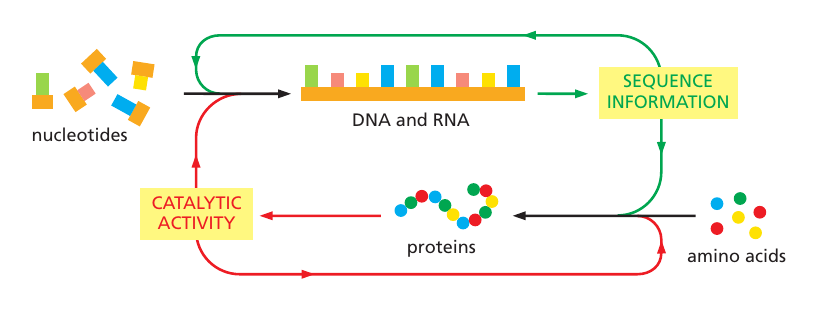
\includegraphics[width=\linewidth]{images/vita-autocatalitica.png}
	\caption{La vita è un processo autocatalitico}\label{fig:awesome_image2}
	\endminipage\hfill
\end{figure}


• codoni, amminoacidi
\subsection{Proteine: le macromolecole più importanti della vita}

\par Oltre agli enzimi ci sono altre proteine importanti, uno degli esempi più noti è l'emoglobina, proteina animale adibita a trasportare ossigeno dai polmoni agli organi e ai tessuti del corpo così come a riportare CO$_{2}$ ai polmoni. 

Importante funzione degli enzimi è correlata alla digestione negli animali. Enzimi come le amilasi e le proteasi sono in grado di ridurre le macromolecole (nella fattispecie amido e proteine) in unità semplici (maltosio e amminoacidi), assorbibili dall'intestino

Tutti gli enzimi sono proteine, ma non tutti i catalizzatori biologici sono enzimi, dal momento che esistono anche catalizzatori costituiti di RNA, chiamati ribozimi

In un organismo, nonostante tutte le cellule condividano gli stessi geni, cellule afferenti a organi o tessuti diversi esprimono geni differenti (\textit{espressione genica}).

\section{Background informatico}

Background informatico
• bioinformatica
• database bioinformatici
• machine learning
• reti neurali, deep learning

\clearpage